\section*{Supplementary note: temporal autocorrelation}
\label{sec:acf}

Headline $H_0$ and $H_1$ tables use the uniform 150-frame rule of
Section~\ref{sec:data}. Supplementary Figure~\ref{fig:acf} is a
diagnostic on the primary match at 1~Hz; it does not choose the stride.
Generate with \texttt{pipeline/steps/09\_acf\_supplement.py}.

\IfFileExists{figures/figS1_acf.pdf}{%
\begin{figure}[h]
\centering
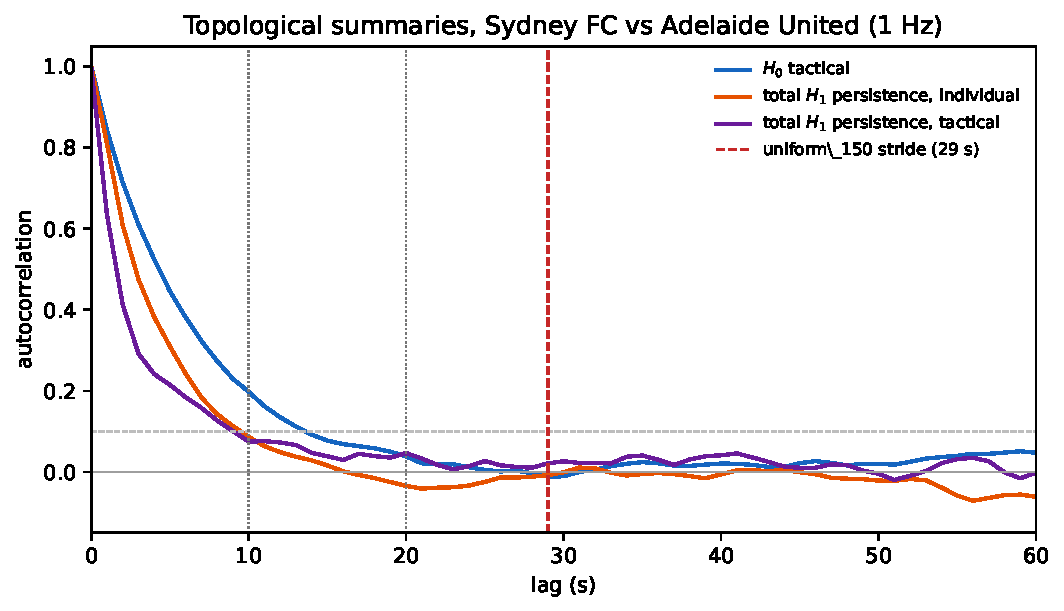
\includegraphics[width=0.85\textwidth]{figures/figS1_acf}
\caption{Autocorrelation of frame-level topological summaries on
SkillCorner match 1996435 at 1~Hz. Series: tactical
\texorpdfstring{$H_0$}{}, and total \texorpdfstring{$H_1$}{}
persistence at the individual and tactical levels. The dashed red line
is the uniform-150 stride.}
\label{fig:acf}
\end{figure}
}{%
\par\textit{Supplementary Figure~S1 is not yet generated. Run
\texttt{09\_acf\_supplement.py} once SkillCorner open data are available.}
\label{fig:acf}
}

\section*{Supplementary Table S1. SkillCorner match identifiers}

Ten A-League matches from the SkillCorner open repository. Home and
away names are those recorded in the tracking files. The primary match
is used for single-match $H_1$ tables, cycle geometry, and
Figure~\ref{fig:acf}.

\begin{table}[h]
\centering
\caption{SkillCorner match identifiers.}
\label{tab:matches}
\begin{tabular}{@{}llll@{}}
\toprule
SkillCorner ID & Home & Away & Role \\
\midrule
1886347 & Auckland FC & Newcastle & multi-match \\
1899585 & Auckland FC & Wellington P FC & multi-match \\
1925299 & Brisbane FC & Perth Glory & multi-match \\
1953632 & CC Mariners & Melbourne City & multi-match \\
1996435 & Sydney FC & Adelaide United & primary \\
2006229 & Melbourne City & Macarthur FC & multi-match \\
2011166 & Wellington P FC & Melbourne V FC & multi-match \\
2013725 & Western United & Sydney FC & multi-match \\
2015213 & Western United & Auckland FC & multi-match \\
2017461 & Melbourne V FC & Auckland FC & multi-match \\
\bottomrule
\end{tabular}
\end{table}
